\documentclass{article}
%-- coding: UTF-8 --
\usepackage[UTF8]{ctex}
\usepackage[utf8]{inputenc}
\usepackage{geometry}
\usepackage{graphicx} % 引入图片
\usepackage{enumitem} % 取消列表默认间距
\usepackage{color}  %导言区调用color宏包
\geometry{left=3.18cm,right=3.18cm,top=2.54cm,bottom=2.54cm}
\usepackage{hyperref}
\hypersetup{hidelinks,
	colorlinks=true,
	allcolors=black,
	pdfstartview=Fit,
	breaklinks=true}
\usepackage{listings}
\usepackage{xcolor}
\usepackage{fontspec}
% 嵌入代码风格
\lstset{
	language    = c++,
	breaklines  = true,
	captionpos  = b,
	tabsize     = 4,
	columns     = fullflexible,
	commentstyle = \color[RGB]{0,128,0},
	keywordstyle = \color[RGB]{0,0,255},
	basicstyle   = \small\ttfamily,
	stringstyle  = \color[RGB]{148,0,209}\ttfamily,
	rulesepcolor = \color{red!20!green!20!blue!20},
	showstringspaces = false,
}



\title{\textbf{实验一 \hspace{0.5cm} 栈、队列与基本排序}}
\author{
\begin{tabular}{c @{\hspace{5mm}} c}
    黄韦杰 & 刘嘉杰 \\  % 作者名
    \href{mailto:hwj@hust.edu.cn}{hwj@hust.edu.cn} & \href{mailto:m202474039@hust.edu.cn}{m202474039@hust.edu.cn} % 邮箱
\end{tabular}
}
\date{September 2024}


\begin{document}
\maketitle

\section{实验项目结构}

\begin{itemize}[noitemsep]
    \item[$-$] project
    \begin{itemize}[noitemsep]
        \item[$-$] include
        \begin{itemize}[noitemsep]
            \item[$\bullet$] dessert.hpp
            \item[$\bullet$] MySort.hpp
            \item[$\bullet$] InsertionSort.hpp
            \item[$\bullet$] MergeSort.hpp
            \item[$\bullet$] MyStack.hpp
        \end{itemize}
        \item[$-$] data
        \begin{itemize}[noitemsep]
            \item[$-$] sample
            \item[$-$] test
            \item[$-$] generate
        \end{itemize}
        \item[$-$] performance
        \begin{itemize}[noitemsep]
            \item[$\bullet$] performance.cpp
        \end{itemize}
        \item[$\bullet$] main.cpp
    \end{itemize}
\end{itemize}

project 文件夹包含了本实验的所有代码源程序以及测试数据。

include 文件夹中, MyStack.hpp 中定义了类 MyStack ; MySort.hpp 头文件定义了 MySort 类,以它为基类在 InsertionSort.hpp 和 MergeSort.hpp 中分别定义了两个子类:InsertionSort 和 MergeSort。\textbf{你需要在本实验中完成 MyStack 、 InsertionSort 和 MergeSort 这三个类的算法实现。}

data 文件夹中包含针对算法程序正确性测试以及性能测试所需的测试数据以及数据生成器。其中,sample 单独用于正确性的检测,仅包含小规模测试集数据,test 用于性能测试,包含部分大规模测试集数据。另外,generate 包含了测试数据的生成器。

performance 文件夹中包含了性能测试的代码。在完成正确性测试之后,可以运行 performance.cpp 来观察两种算法的性能。

main.cpp 是正确性检测的主程序,当你编写完 InsertionSort.hpp 、 MergeSort.hpp 或者 MyStack.hpp 后,可以编译运行 main.cpp ,测试你程序的正确性。

\textcolor{red}{在本地运行没有问题后,请将代码提交到Online Judge上,可以多次提交,实时查看得分情况,实验的最终成绩以OJ上的作业完成情况以及提交的实验报告为准。}

\section{实验内容}

\subsection{栈}

根据栈数据结构的思想,完成 MyStack.hpp 中的代码。并通过运行 main.cpp 的正确性检测。

\begin{lstlisting}
    class MyStack {
        public:
            ElementType elem[MAXLENG]; // 模拟栈的静态数组
            int top; // 栈顶指针, 注意本实现的顶元素为elem[top]!

            // 初始化静态栈
            // 本函数不需修改
            void Initstack() {
                memset(elem, -1, sizeof elem);
                top = -1;
            }

            // 判断栈空, 若为空栈,则Empty()返回true;否则返回false
            bool Empty() {
                // 请在这里完成你的代码
            }

            // 判断栈满,若栈满,则Full()为true;否则为false
            bool Full() {
                // 请在这里完成你的代码
            }

            // 元素e进栈,若栈满,则无法成功插入,插入成功返回true,否则返回false
            // @param
            // e: 将要入栈的元素
            bool Push(ElementType e) {
                // 请在这里完成你的代码
            }

            // 栈的顶元素拷贝到e,若栈为空,则无法拷贝,返回false,成功拷贝则返回true
            // @param
            // e: 指向存放栈顶元素地址的指针
            bool Gettop(ElementType &e) {
                // 请在这里完成你的代码
            }

            // 删除栈s的顶元素,并将删除的元素赋给e带出,若栈空,则无法成功删除,删除成功返回true,否则返回false
            // @param
            // e: 指向存放出栈元素地址的指针
            bool Pop(ElementType &e) {
                // 请在这里完成你的代码
            }
    };
\end{lstlisting}

具体来说,你需要对通过数组模拟栈,并实现栈相关的基本操作 elem 数组实际存储着栈中的数据, top 为 elem 中栈顶元素的序号。

Empty 为判断栈中是否为空的函数,在栈中没有元素时返回 true ,否则返回 false 。

Full 为判断栈是否已被填满的函数,在栈被填满的情况下返回 true ,否则返回 false 。

Push 函数将新元素插入栈顶,插入成功则返回 true ,插入失败(如栈已被填满)则返回 false 。

Gettop 函数拷贝出栈顶元素,拷贝成功则返回 true ,拷贝失败(如栈为空)则返回 false 。

Pop 函数取出栈顶元素并将原来位置的元素删除,取出成功则返回 true ,取出失败(如栈为空)则返回 false 。

编写代码之后,你可以运行 main.cpp 进行测试,如果正确的话,会出现下图中的结果。


\begin{figure}[h]
\centering
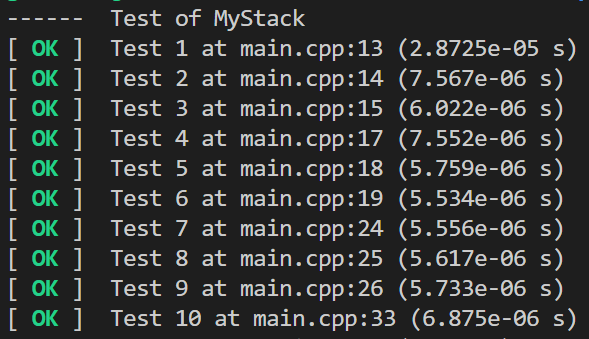
\includegraphics[width=8cm]{img/lab1/insertionsort.png}
\end{figure}

\subsection{选择排序}

根据插入排序的思想,完成 InsertionSort.hpp 中的代码。并通过编译运行 main.cpp 的正确性检测。

\begin{lstlisting}
    class InsertionSort: public MySort {
    public:
        // 通过插入排序对int队列nums进行升序排序
        // @param
        // nums: 完整的待排序队列,最终排序的结果应存放在nums中
        void mysort(std::vector<int>& nums) {
            // 请在这里完成你的代码
        }
    };
\end{lstlisting}

具体来说,你需要对 nums 中的数字使用选择排序算法进行排序。mysort 并不需要返回任何内容,因为参数 nums 为引用传递,在函数内部对 nums 的修改会对调用该函数时传入的实参产生影响。


\subsection{归并排序}

根据归并排序的思想,完成 MergeSort.hpp 中的代码。并通过运行 main.cpp 的正确性检测。

\begin{lstlisting}
    class MergeSort: public MySort {
    public:
        // 通过归并排序对int队列nums中的[left, right]区间进行升序排序
        // @param
        // nums: 完整的待排序队列,最终排序的结果应存放在nums中
        // left: 当前排序区间的左端点
        // right: 当前排序区间的右端点
        void merge_sort_aux(std::vector<int>& nums, int left, int right) {
            // 请在这里完成你的代码
        }
        void mysort(std::vector<int>& nums) {
            int n = nums.size();
            merge_sort_aux(nums, 0, n - 1);
        }
    };
\end{lstlisting}

具体来说,你需要对 nums 中的数字使用归并排序算法进行排序。mysort 并不需要返回任何内容,因为参数 nums 为引用传递,在函数内部对 nums 的修改会对调用该函数时传入的实参产生影响。

merge\_sort\_aux 函数为归并排序辅助函数,你需要对 nums 数组闭区间 [left, right] 内的数值进行排序。



\section{实验思考}
\begin{enumerate}
    \item 以第一组测试数据为例,分别观察选择排序和归并排序过程中数组元素的变化情况(需要逐步给出)。
    \begin{itemize}
        \item input \\ 5 \\ 1 6 2 10 2
        \item output \\ 1 2 2 6 10
    \end{itemize}
    
    \item 比较插入排序与归并排序的性能差距。
    \item 【拓展题】
    \begin{itemize}
        \item 尝试修改源代码,实现排序过程中「比较」操作的计数功能,并以该角度来对插入排序和归并排序进行对比。
        \item 不基于比较操作,如何实现排序。
    \end{itemize}

    \item 【拓展题】基于归并排序,求解给定数组的逆序对问题。
    在数组中的两个数字,如果前面一个数字大于后面的数字,则这两个数字组成一个逆序对。
    输入一个数组,求出这个数组中的逆序对的总数。
    \begin{itemize}
        \item input \\ 4 \\ 7 5 6 4
        \item output \\ 5
    \end{itemize}
    
\end{enumerate}

\end{document}